\chapter{Introduction}

Le but de ce projet est de développer une plateforme de signalement pour la maintenance des
infrastructures d'une organisation. Cette plateforme permettra aux usagers de signaler une
anomalie sur une ressource simplement en scannant un QR code.

\section{Exigences fonctionnelles}

On pourra distinguer trois types d'utilisateurs sur cette plateforme :
\begin{itemize}
    \item Les utilisateurs anonymes qui peuvent signaler des anomalies en flashant le QR associé
        à une ressource et en décrivant l'anomalie.
    \item Les responsables de maintenance qui peuvent gérer les ressources et les tickets
        d'anomalies. Chaque responsable possèdent un ensemble de ressources dont ils sont les
        seuls à s'occuper.
    \item Enfin, un administrateur (unique) qui peut gérer les responsables de maintenance et
        transférer les droits sur les ressources.
\end{itemize}
\medskip

Pour chaque ressource un utilisateur pourra déclarer une nouvelle anomalie ou bien séléctionner
une parmi une listes d'anomalies déjà entrée par les autres utilisateurs.\newline

On devra pouvoir imprimer sur la plateforme les étiquettes avec les QR code et les URLs 
correspondant aux ressources. Les étiquettes devront avoir un format de 105x42 mm une fois
imprimées et l'impression devra ce faire depuis un rendu Web sans générer de PDF.

\chapter{Architecture}
Cette section détaille l'architecture que nous avons choisi pour créer la plateforme.

Elle explique aussi les choix de technologies que nous avons fait et le déroulement du
développement dans les grandes lignes.

\section{Modèle de la base de données}
La première étape de la conception était de décider du modèle de la base de données. Le schéma
suivant décrit le schéma des tables que nous avons choisi :\newline

\begin{figure}[!h]
    \centering
    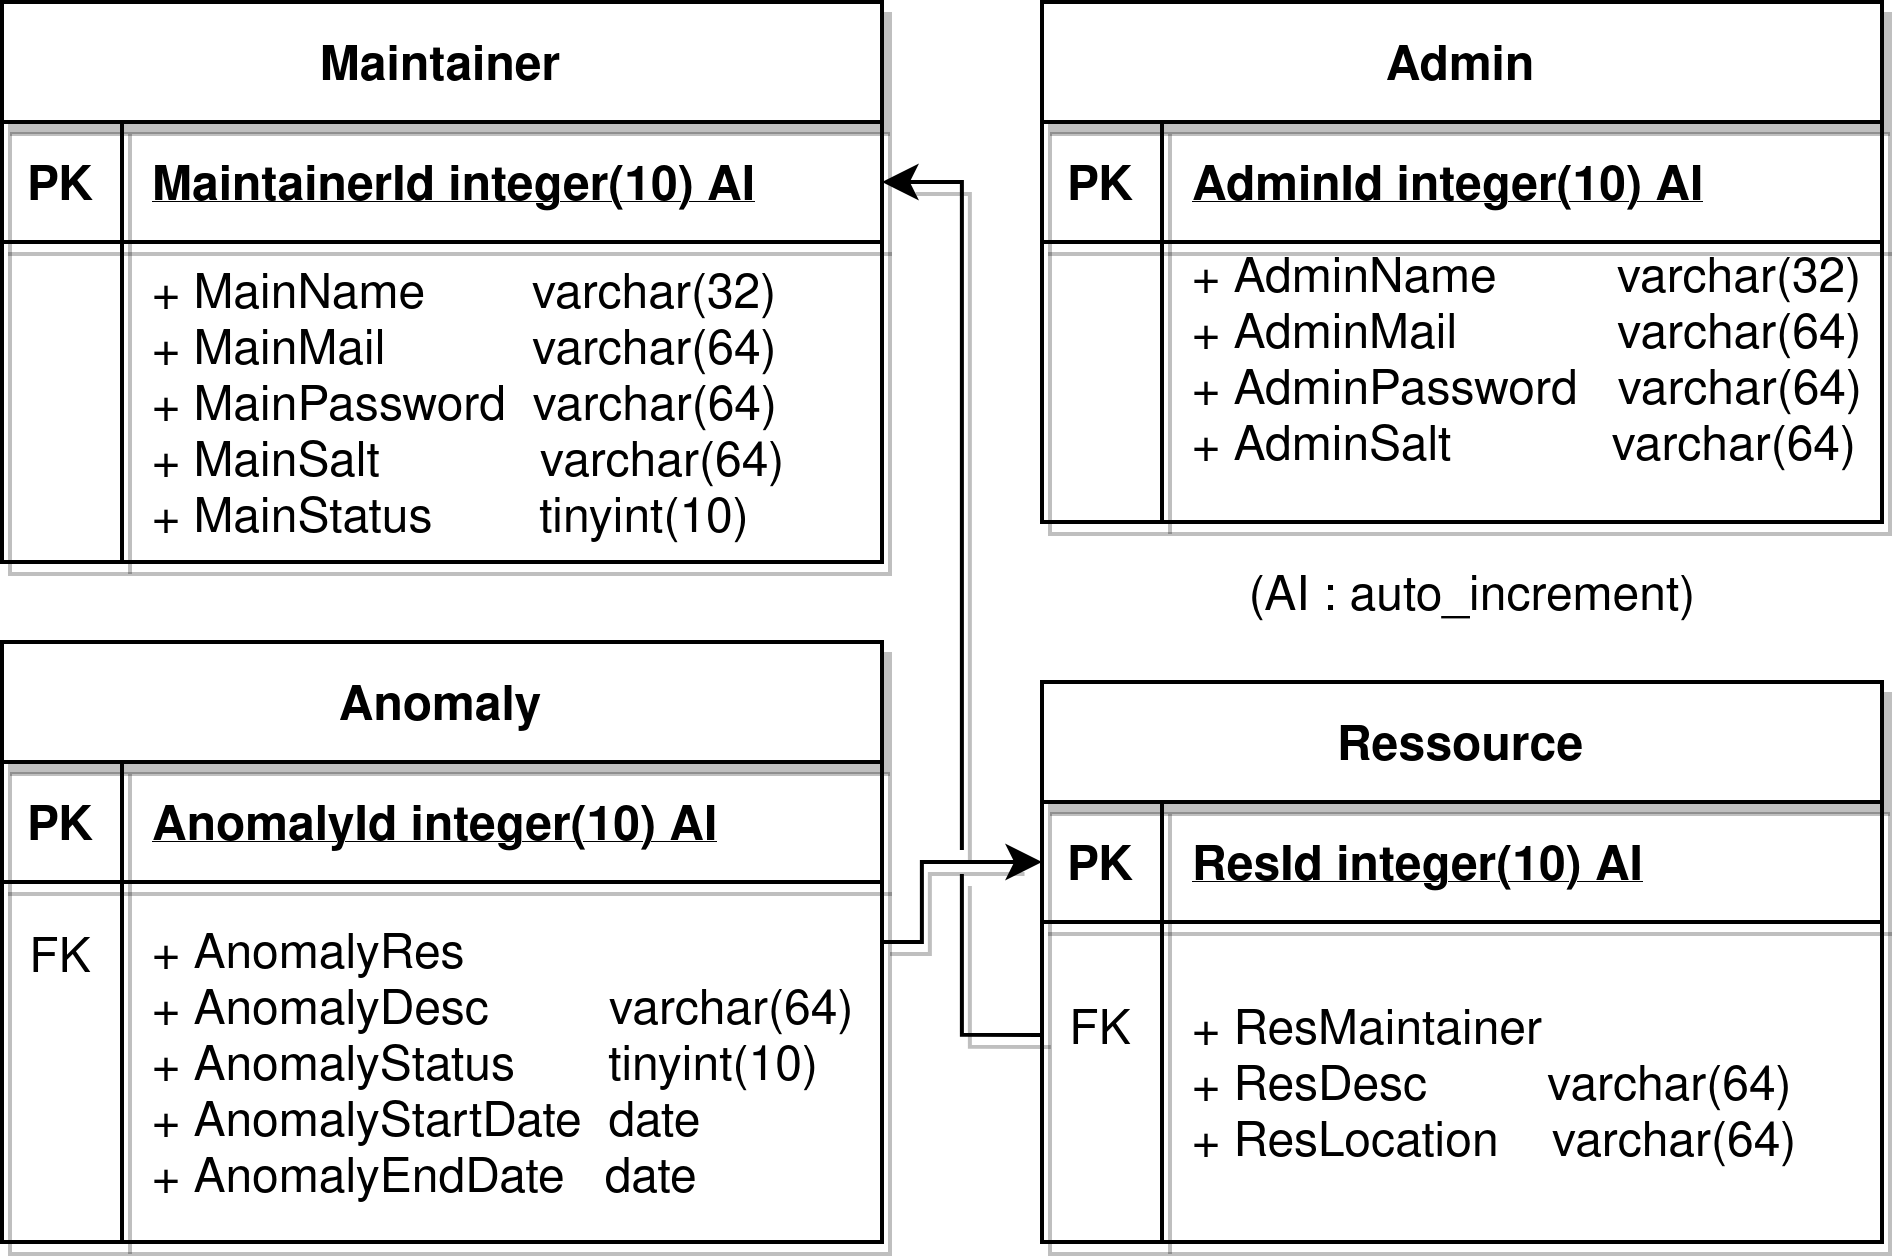
\includegraphics[width=\textwidth]{img/schemaSQL.png}
    \caption{Schéma des tables de la base de données}
    \label{fig:schemaSQL}
\end{figure}
\newpage

\section{Technologies choisies}
La partie vue est écrite dans les langages classiques : HTML \& CSS. Nous n'avons (quasiment) pas
utiliser de JavaScript pour la plateforme.\newline

Nous avons choisis d'utiliser Java avec les Servlets et les JSP pour développer la partie
contrôleur de l'application.\newline

Le modèle est donc écrit en Java en utilisant la bibliothèque JDBC pour les interactions avec
le SGBD (MySQL).

\subsection{Frameworks}
Pour développer la plateforme nous avons utilisés un framework pour le CSS :
\textbf{Bootstrap}.
Cela nous a permis de simplifier grandement le développement du front-end afin de se concentrer
sur le back-end.

\section{Modèle}

L'application a été conçu en suivant le modèle MVC (Modèle-Vue-Contrôleur). C'est le modèle le
plus simple et le plus utilisée et également celui que l'on a vu en cours donc c'était un choix
évident.\newline

Nous avons premièrement implémenter des classes Java décrivant simplement le
modèle des types d'objets utilisés, c'est-à-dire :
\begin{itemize}
    \item \verb:User: : classe des utilisateurs,
    \item \verb:Admin: : classe des administrateurs, héritant de \verb:User:,
    \item \verb:Maintainer: : classe des responsables de maintenance, héritant de \verb:User:,
    \item \verb:Ressource: : classe des ressources,
    \item \verb:Anomaly: : classe des anomalies.
\end{itemize}
\medskip

Ensuite pour chacune des classes exceptées \verb:User: nous avons écrit une classe correspondante
qui fait l'intermédiaire entre le SGBD et le modèle, selon le modèle DAO (Data Access Object).
\newline

Les DAO nous permettent donc de récupérer un élément de la base de donnée directement sous forme
d'objets du modèle. Ensuite nous pouvons donc facilement manipuler ces objets à notre guise puis
si besoin les renvoyer au DAO afin de mettre à jour la base de données selon l'état de cet objet.

Un exemple d'utilisation du DAO est illustré avec la figure \ref{fig:dao}.

\begin{figure}[h]
    \centering
    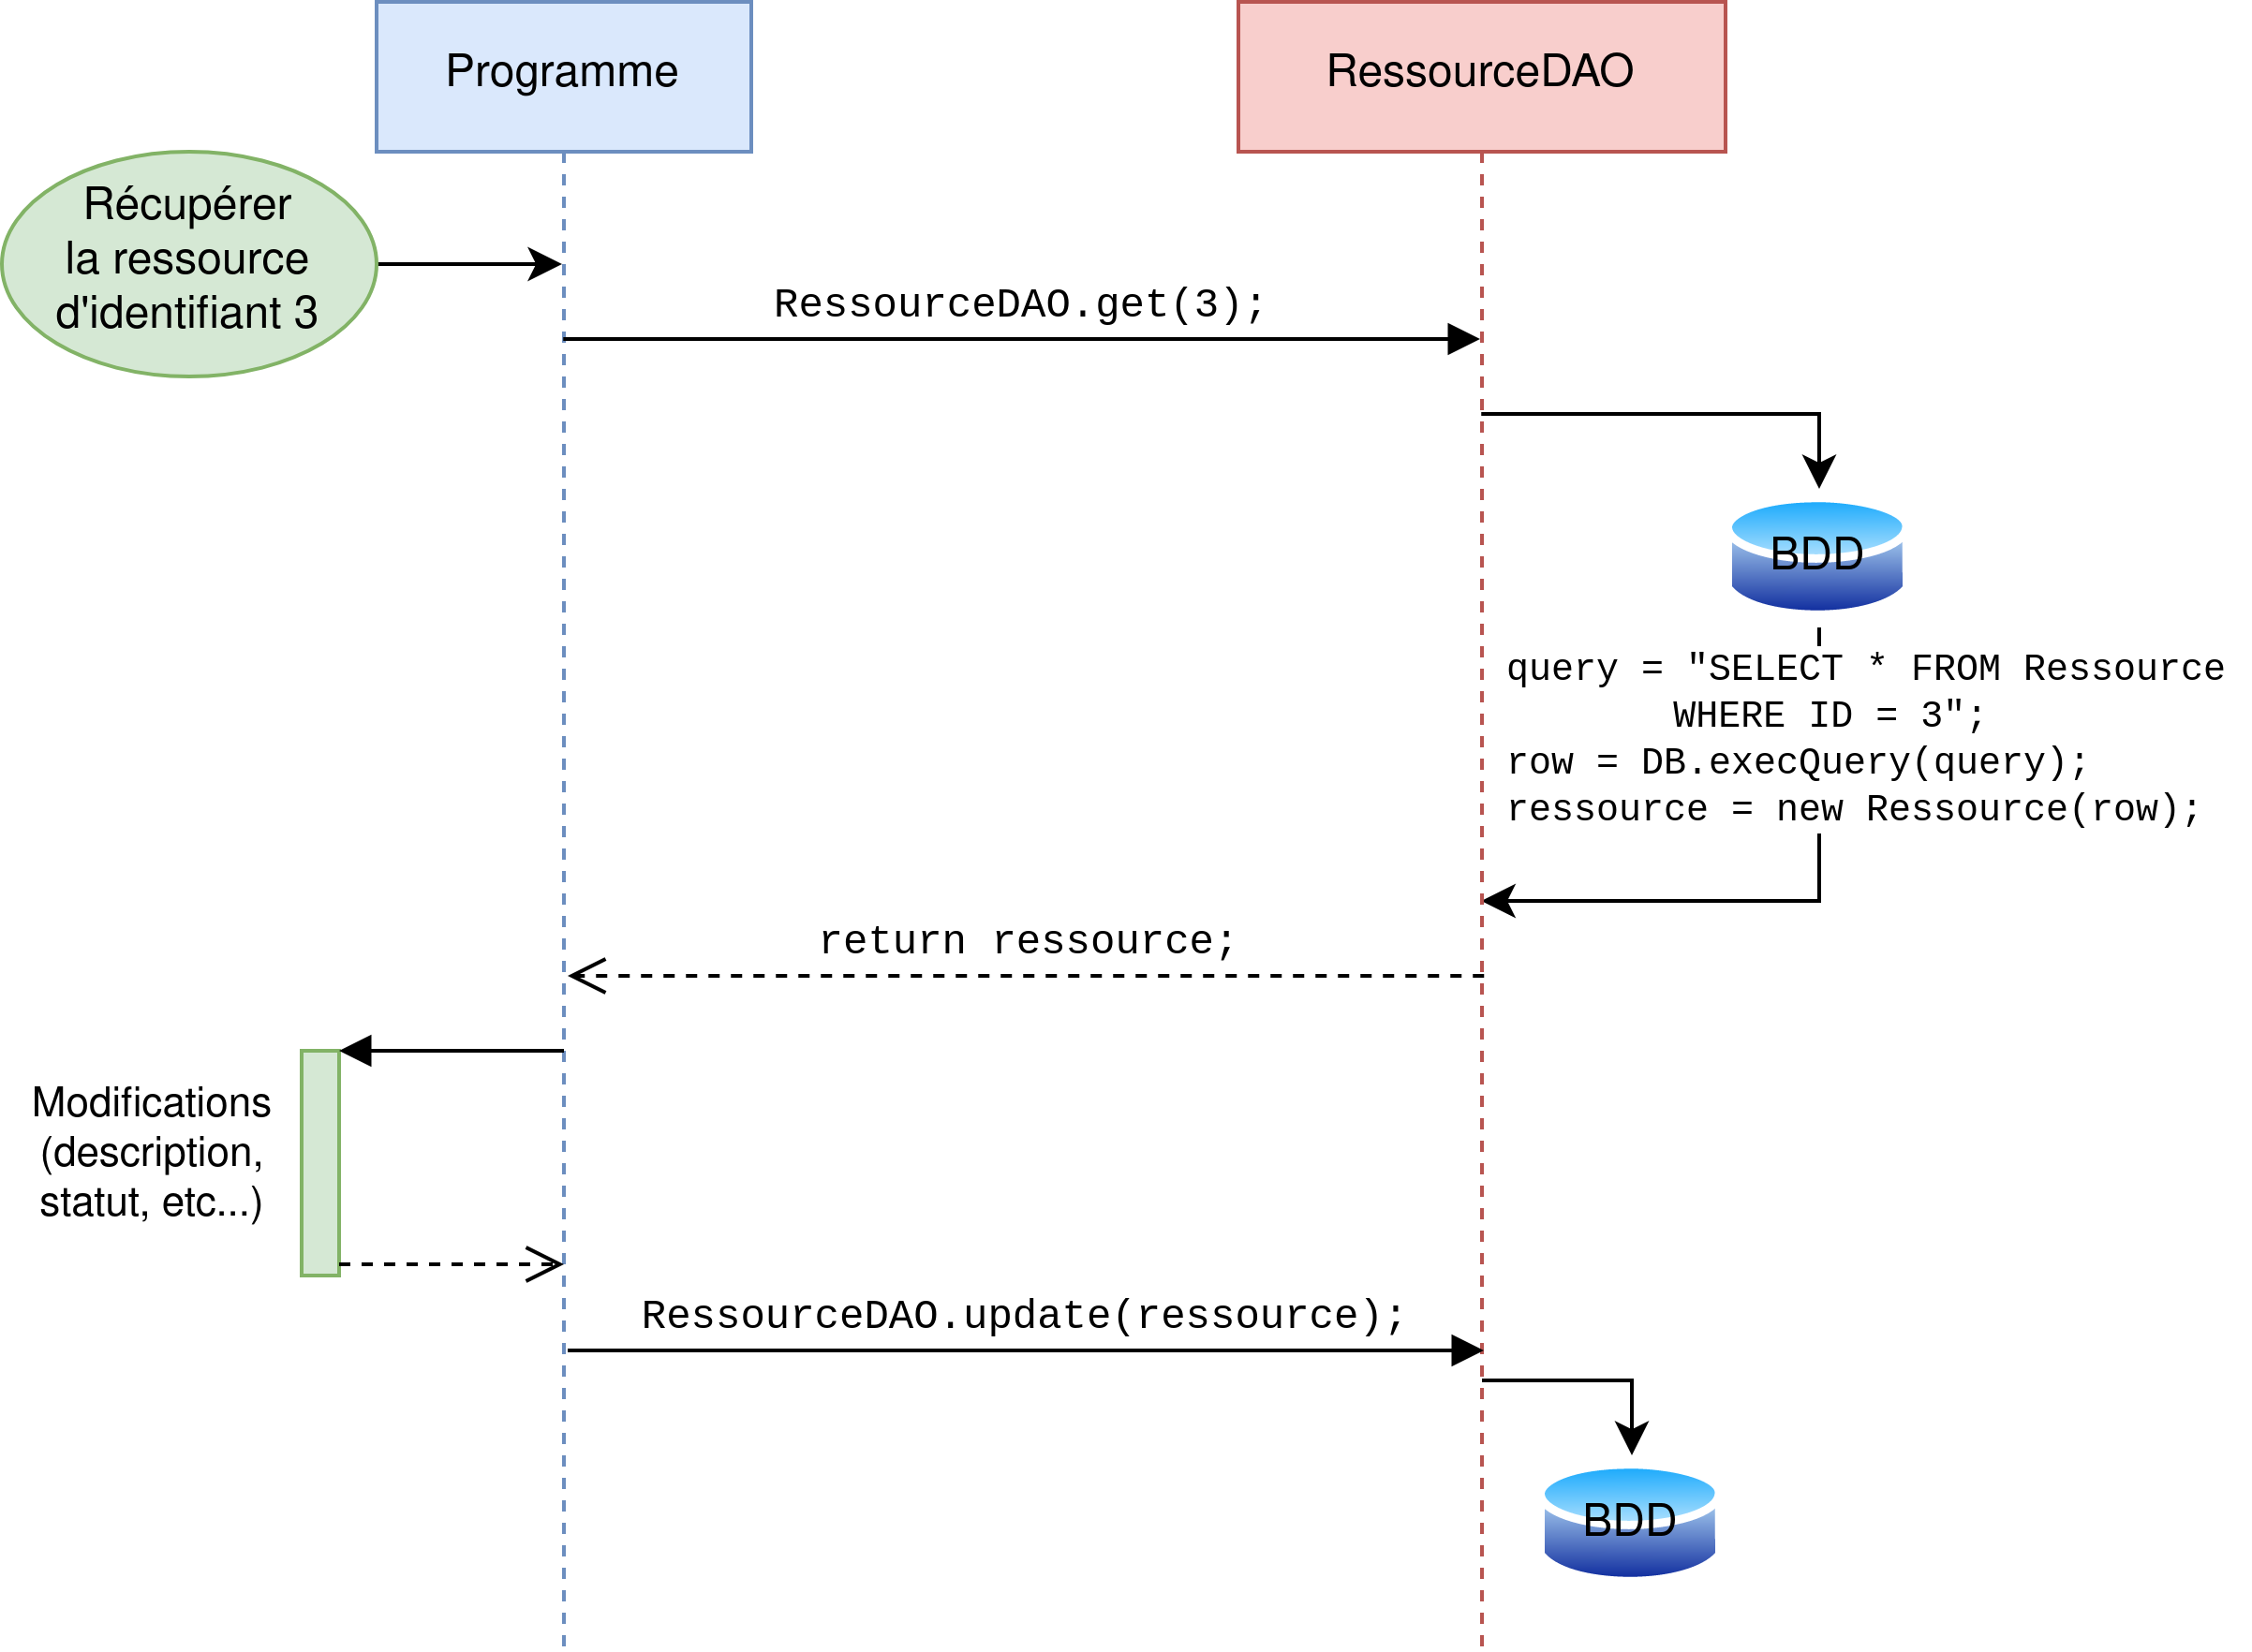
\includegraphics[width=\textwidth]{img/DAO.png}
    \caption{Exemple d'utilisation de la classe RessourceDAO}
    \label{fig:dao}
\end{figure}
\newpage
\medskip

\section{Sécurisation}

Afin de sécuriser au mieux la plateforme nous avons mis en place les sécurités suivantes :
\begin{description}
    \item[\textbf{Filtrage des urls:}] via un filter JEE.
    \item[\textbf{Requête préparées:}] en utilisant la bibliothèque JDBC.
    \item[\textbf{Encodage des caractères spéciaux:}] afin d'éviter des injections XSS
\end{description}
\medskip

Une fois ses différentes sécuritées mises en place, nous avons testé leurs fiabilités en essayant
d'effectuer différentes actions :
\begin{itemize}
    \item Obtenir sur la plateforme des droits que nous avons pas (broken access control).
    \item Injections XSS.
    \item Injections SQL.
\end{itemize}
\newpage

\subsection{Stockage des mots de passe}

Pour pouvoir stocker les mots de passe de manière sécurisée, nous avons procédé de la manière
suivante :
\begin{enumerate}
    \item Pour chaque utilisateur on génère un sel en utilisant le CSPRNG (Cryptographically Strong
        Pseudo Random Number Generator) de Java (\verb:SecureRandom:). Ce sel est une suite de
        bits que l'on encode ensuite en base64 (pour le stockage dans la BDD).

    \item Ensuite on converti le mot de passe de l'utilisateur en bits et on décode notre sel. On
        peut maintenant hashé notre suite de bits composé du sel et du mot de passe. Pour cela on
        utilise la classe \verb:MessageDigest: de Java avec l'algorithme SHA-256.

    \item Une fois le hash généré on peut ré-encoder celui ci en base64 et le stocker ainsi que le
        sel dans la base de donnée.
\end{enumerate}

Pour vérifier un mot de passe lors d'une connexion il suffit de récupérer le sel dans la base
de données et de refaire l'étape 2. Ensuite on compare simplement la chaîne ainsi créée avec le
mot de passe de référence dans la BDD.

\subsection{Statut des responsables de maintenance}

Comme la page de création de compte est accessible par tous, pour faire en sorte que n'importe
quel utilisateur n'obtienne pas les droits d'un responsable de maintenance, nous avons défini
un attribut supplémentaire : le statut (\verb:MainStatus:).

Il est par défaut défini à <<en attente>>, c'est-à-dire en attente de validation par
l'administrateur. Ensuite si l'administrateur l'active il passe à <<actif>>, à ce moment là le
responsable obtient ses droits, puis peut repasser à <<inactif>> si l'administrateur le décide.

\chapter{Difficultés}

Durant ce projet nous avons eu des difficultés qui ont fait que celui ci nous as pris beaucoup
plus de temps que prévu.\newline

La première difficulté fut de réussir à interagir avec notre base de données en utilisant Java.
Après quelques échecs et des recherches sur Internet nous avons trouvé le problème : l'ensemble
de classes qui permet les interactions avec un SGBD (JDBC) n'est pas intégré à l'API Java de
base. Il fallait donc trouver, télécharger et inclure au projet la librairie le permettant
(\verb:mysql-connector-java.jar:).\newline

Après avoir écrit le modèle et la vue du projet, nous avons eu quelques difficultés au moment
d'écrire le contrôleur :
\begin{itemize}
    \item Comprendre le mapping entre les différentes routes et les contrôleurs Java associés,
        et comment le définir dans le fichier \verb:web.xml:.
    \item Arriver à structurer le contrôleur de manière épuré et factoriser le code.
    \item La différence entre les appels \verb:requestDispatcher.forward: et\\
        \verb:HttpServletResponse.sendRedirect:.
    \item Éviter les broken access control.
    \item Comprendre le fonctionnement et la mise en place des \verb:servlet.Filter:.
\end{itemize}
\medskip

Également le fait d'utiliser Java comme langage de programmation de la plateforme nous as
poussé à utiliser Eclipse comme IDE. Cela permet de gagner beaucoup de temps sur certains points
(compilation, tests, auto-complétion, vérification de la syntaxe) mais aussi nous en as fait
perdre énormément à causes de problèmes pour ajouter des librairies, des différentes versions
et de leurs compatibilités, de bugs etc...

Aussi, le fait d'utiliser un IDE aussi puissant avec beaucoup d'outils qui permet de se passer de
certaines tâches comme Eclipse fait que nous ne connaissons pas tout le fonctionnement derrière.
Et donc, pour une tâche comme le déploiement du site sur la VM, nous avons eu des problème. Par
exemple, les librairies externes ne se liaient pas correctement, nous avons cherché longtemps
avant de comprendre qu'il fallait les copier dans un répertoire spécifique et redémarrer Tomcat
(voir \verb:install.sh:).


\chapter{Conclusion}
En conclusion, malgré les difficultés rencontrées, nous avons pu terminer le projet, et celui-ci
est fonctionnel. Les différentes exigences et contraintes ont été respectées.

Ce projet nous as permis de mieux comprendre l'architecture d'une application Web, le modèle
MVC et la sécurisation de celle-ci. Également il nous as fait manipuler les Servlets et JSPs
qui facilite beaucoup l'implémentation d'une application en suivant le modèle MVC.

\chapter{Annexe}

\section{Notice d'installation}

L'installation peut se faire de deux manières différentes :

\begin{enumerate}
    \item Premièrement, copier l'archive \verb:install.tar.gz: sur la machine cible, ensuite
        l'extraire puis lancer le script \verb:install.sh: avec les droits administrateurs.

    \item Sinon l'application peut être installer directement depuis la machine cible en recupérant
        le script d'installation sur GitHub et en lançant le script comme precédemment :
\end{enumerate}

\begin{minted}{bash}
wget https://raw.githubusercontent.com/loukabvn/projet-web/main/install.sh
chmod u+x install.sh
su root
./install.sh
\end{minted}

Il faut ensuite renseigner les informations demandées c'est-à-dire les identifiants pour le
compte MySQL pour l'accès administrateur à la base de données (1) et les identifiants pour le compte
administrateur de la plateforme (2).

Une fois l'installation terminée vous pouvez vous rendre sur :
\begin{center}
    \label{url:home}
    \url{http://192.168.76.76:8080/ProjetWeb/home}
\end{center}
et vous connecter avec les identifiants renseignés (2).

\section{Jeu de données}

Un jeu de données pré-rempli est disponible pour effectuer des tests sur notre plateforme.
Pour pouvoir utiliser ces données il suffit d'exécuter avec mysql le script \verb:insertion.sql:.
Également, durant l'installation, l'insertion de ce jeu de données de test vous ait proposé, que
vous pouvez accepter ou refuser.
\newpage

\section{Utilisation}

Après avoir installé la plateforme et créé le compte de l'administrateur vous pouvez vous rendre
sur le lien précédent (section \ref{url:home}). Vous arrivez sur la page suivante :

\begin{figure}[!h]
    \centering
    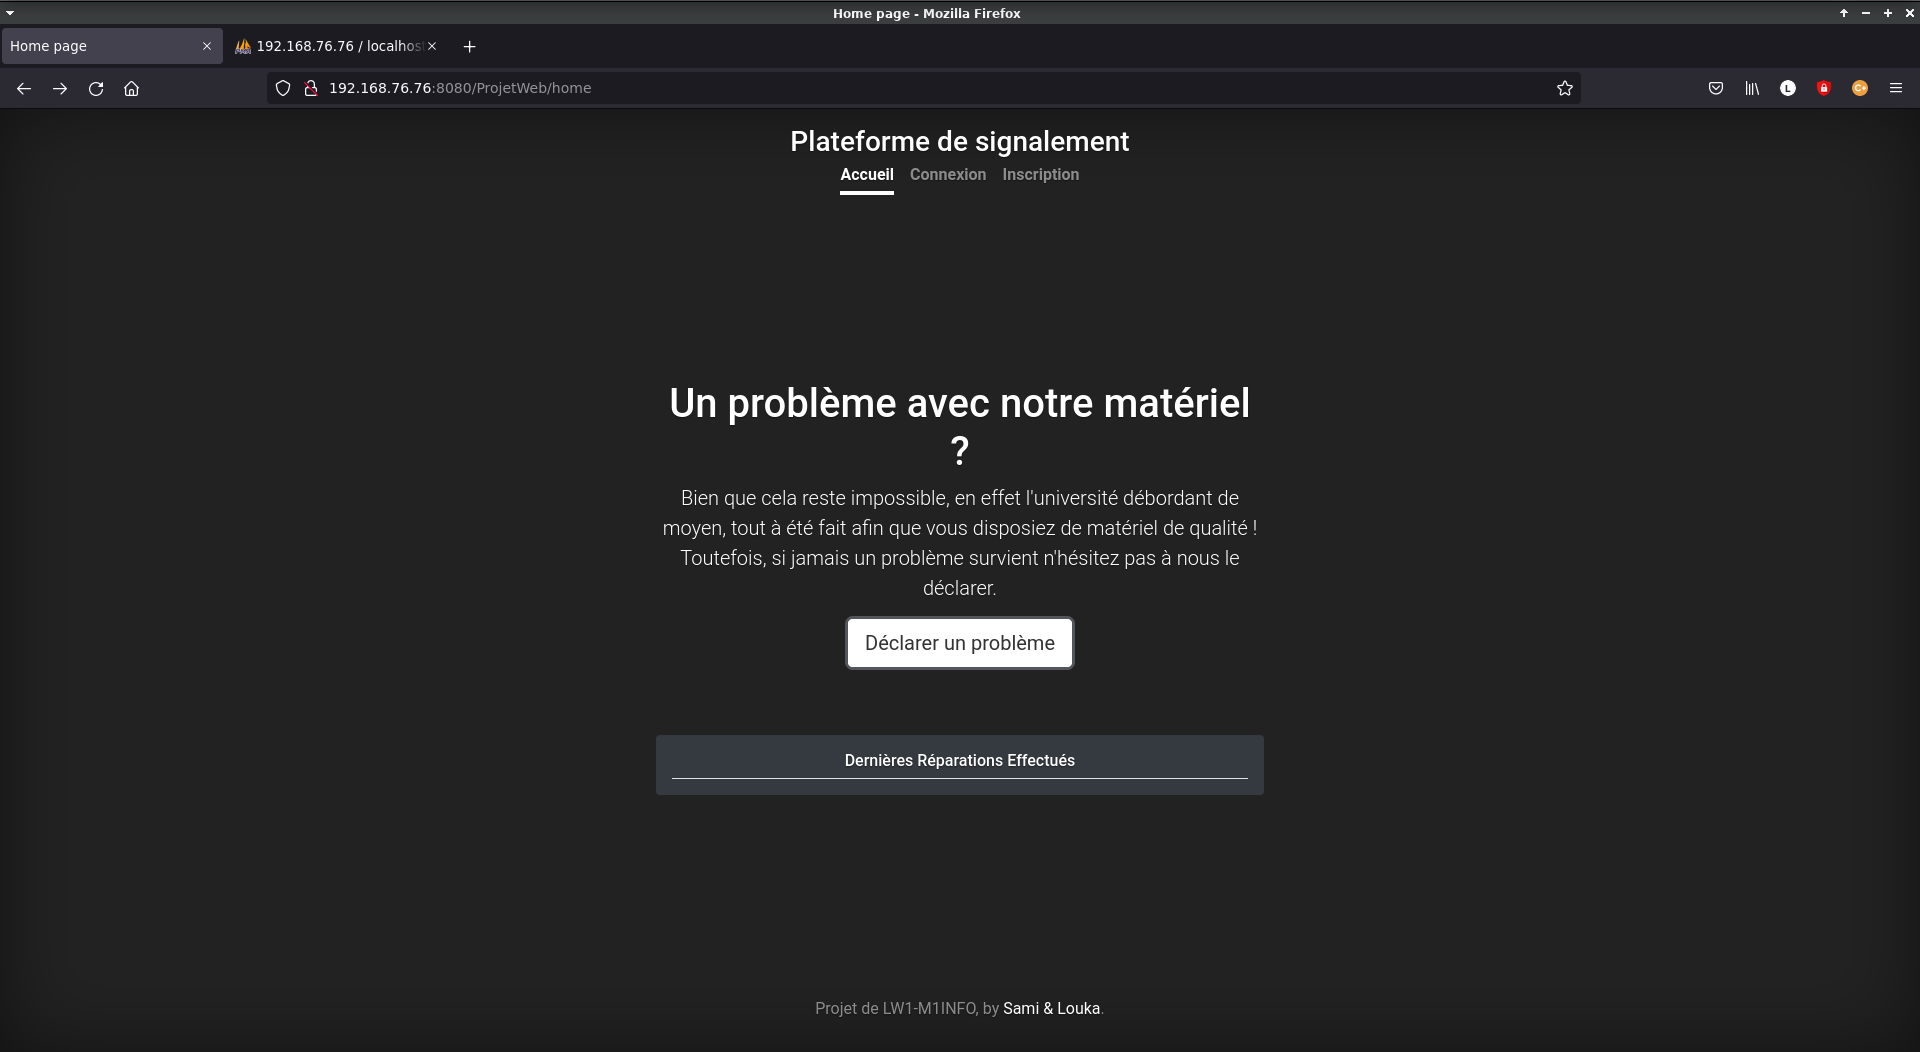
\includegraphics[width=15cm]{img/home.png}
    \caption{Accueil du site}
\end{figure}

Vous pouvez ensuite vous connecter en cliquant sur \textbf{Connexion}. La page suivante
s'affichera :
\begin{figure}[!h]
    \centering
    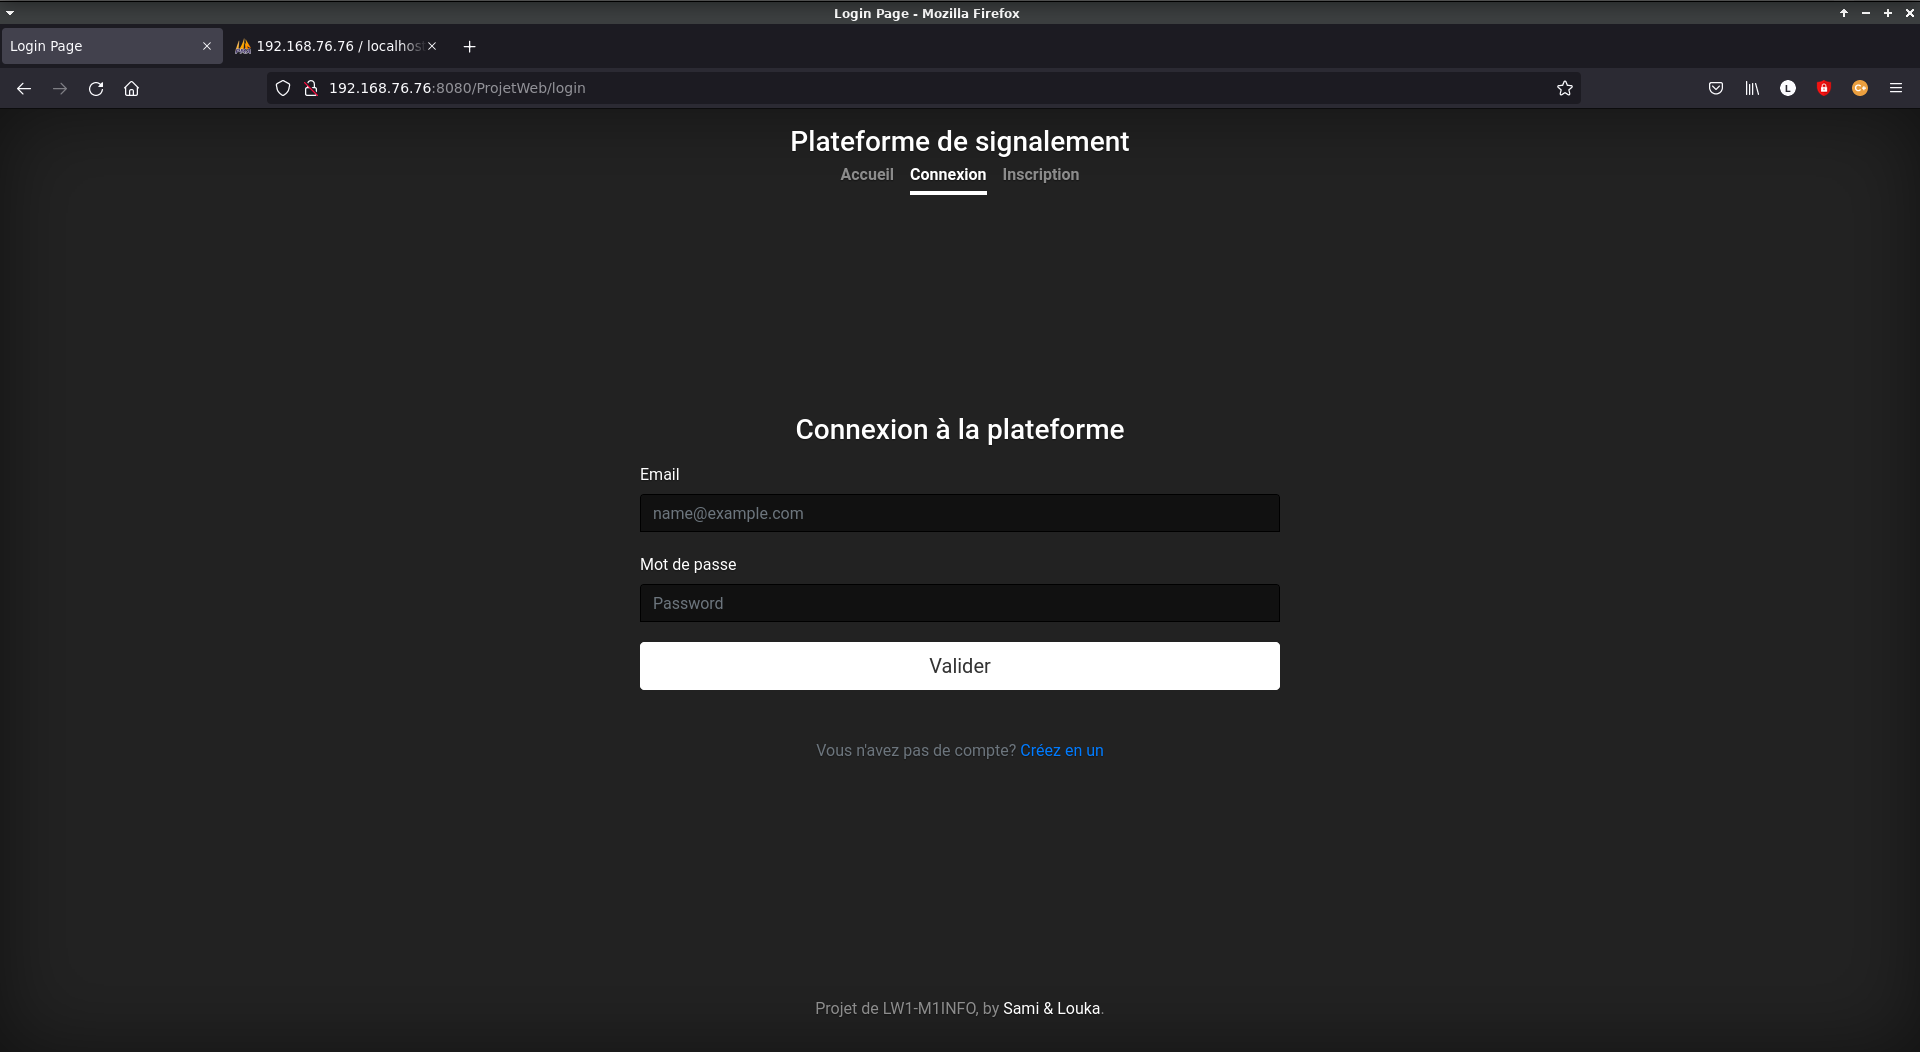
\includegraphics[width=15cm]{img/sign-in.png}
    \caption{Page de connexion}
\end{figure}
\newpage

Lorsque vous vous connecter en tant qu'administrateur vous arrivez sur la page suivante :
\begin{figure}[!h]
    \centering
    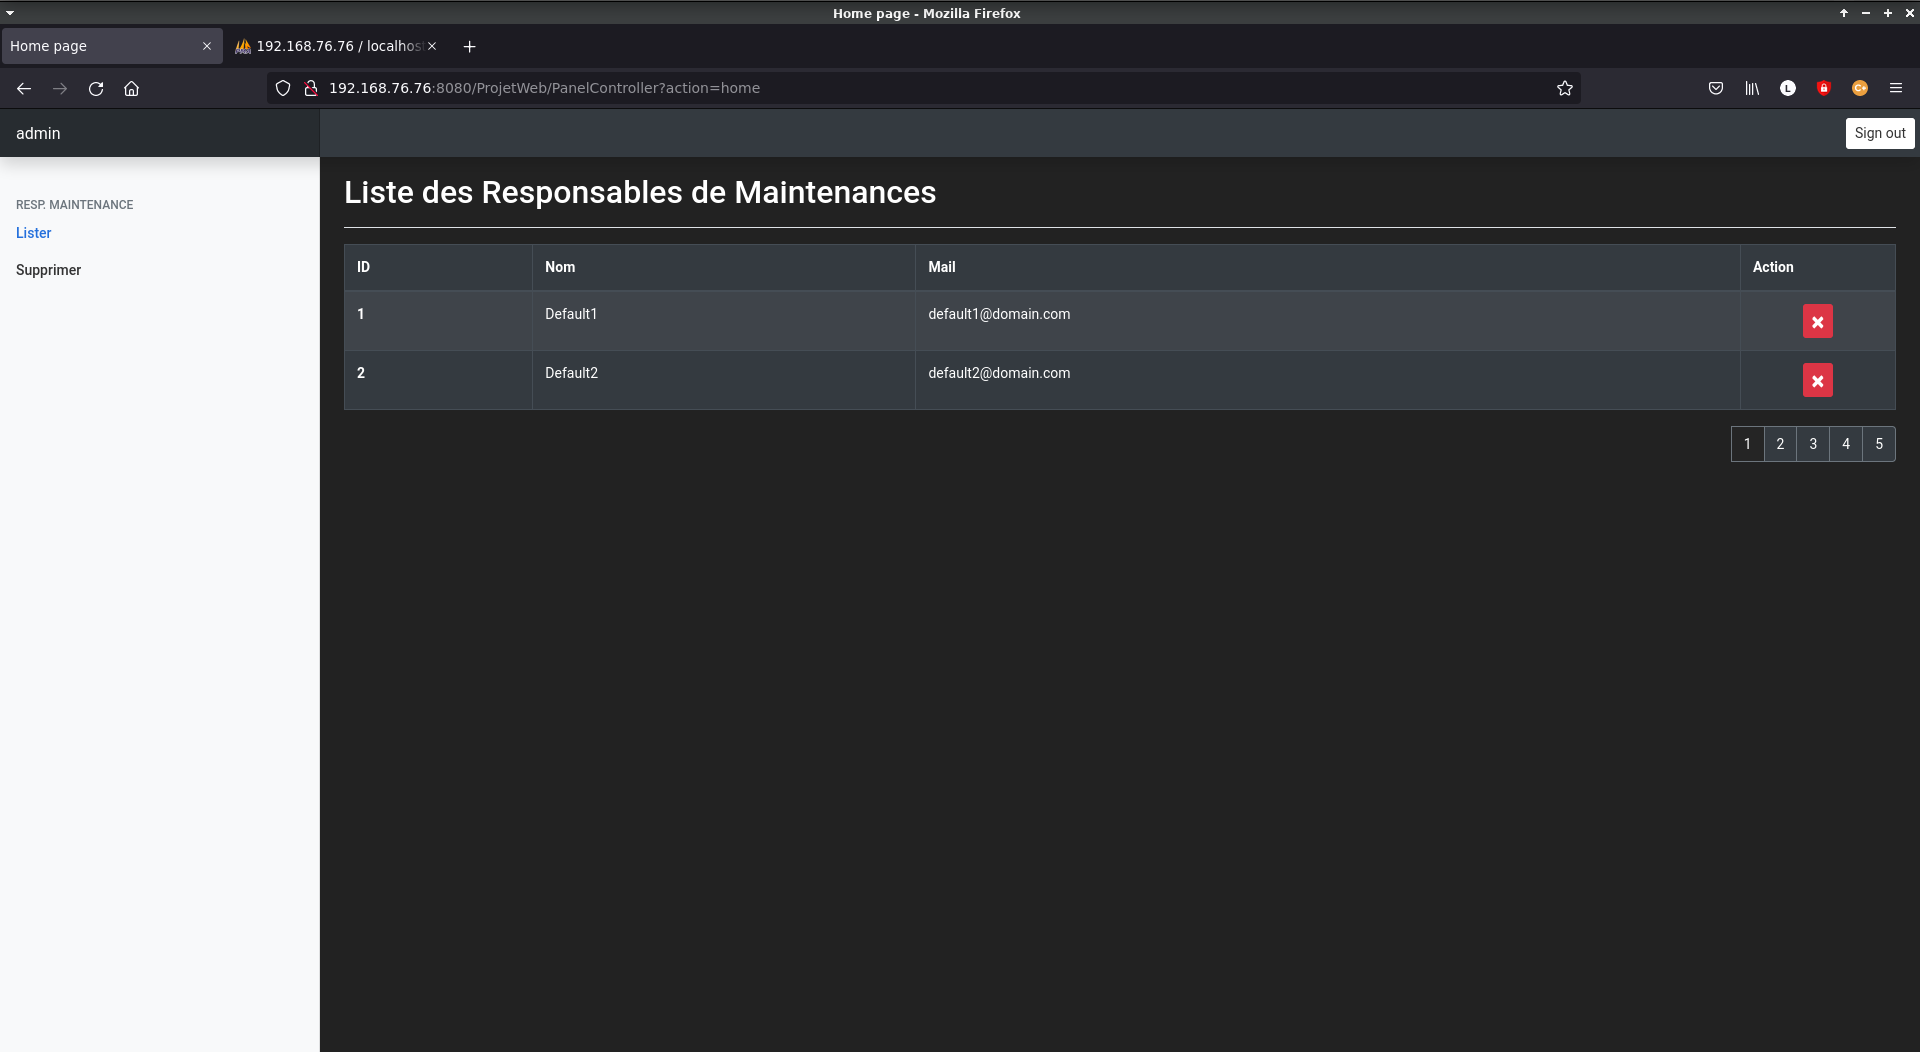
\includegraphics[width=\textwidth]{img/admin.png}
    \caption{Panneau administrateur}
\end{figure}

Dans le panneau latéral, on peut effectuer les actions suivantes :
\begin{description}
    \item[\textbf{Lister}] : permet de lister les responsables de maintenance, de voir et modifier
        leurs statuts : en attente / actif / inactif (bouton rouge à gauche de chaque responsable).
    \item[\textbf{Supprimer}] : permet de supprimer un responsable de maintenance et de donner les
        ressources dont il est responsable à un autre responsable.
\end{description}
\newpage

Ensuite, pour créer un compte de responsable de maintenance il faut se rendre sur la page
d'enregistrement en cliquant sur \textbf{Inscription} :
\begin{figure}[!h]
    \centering
    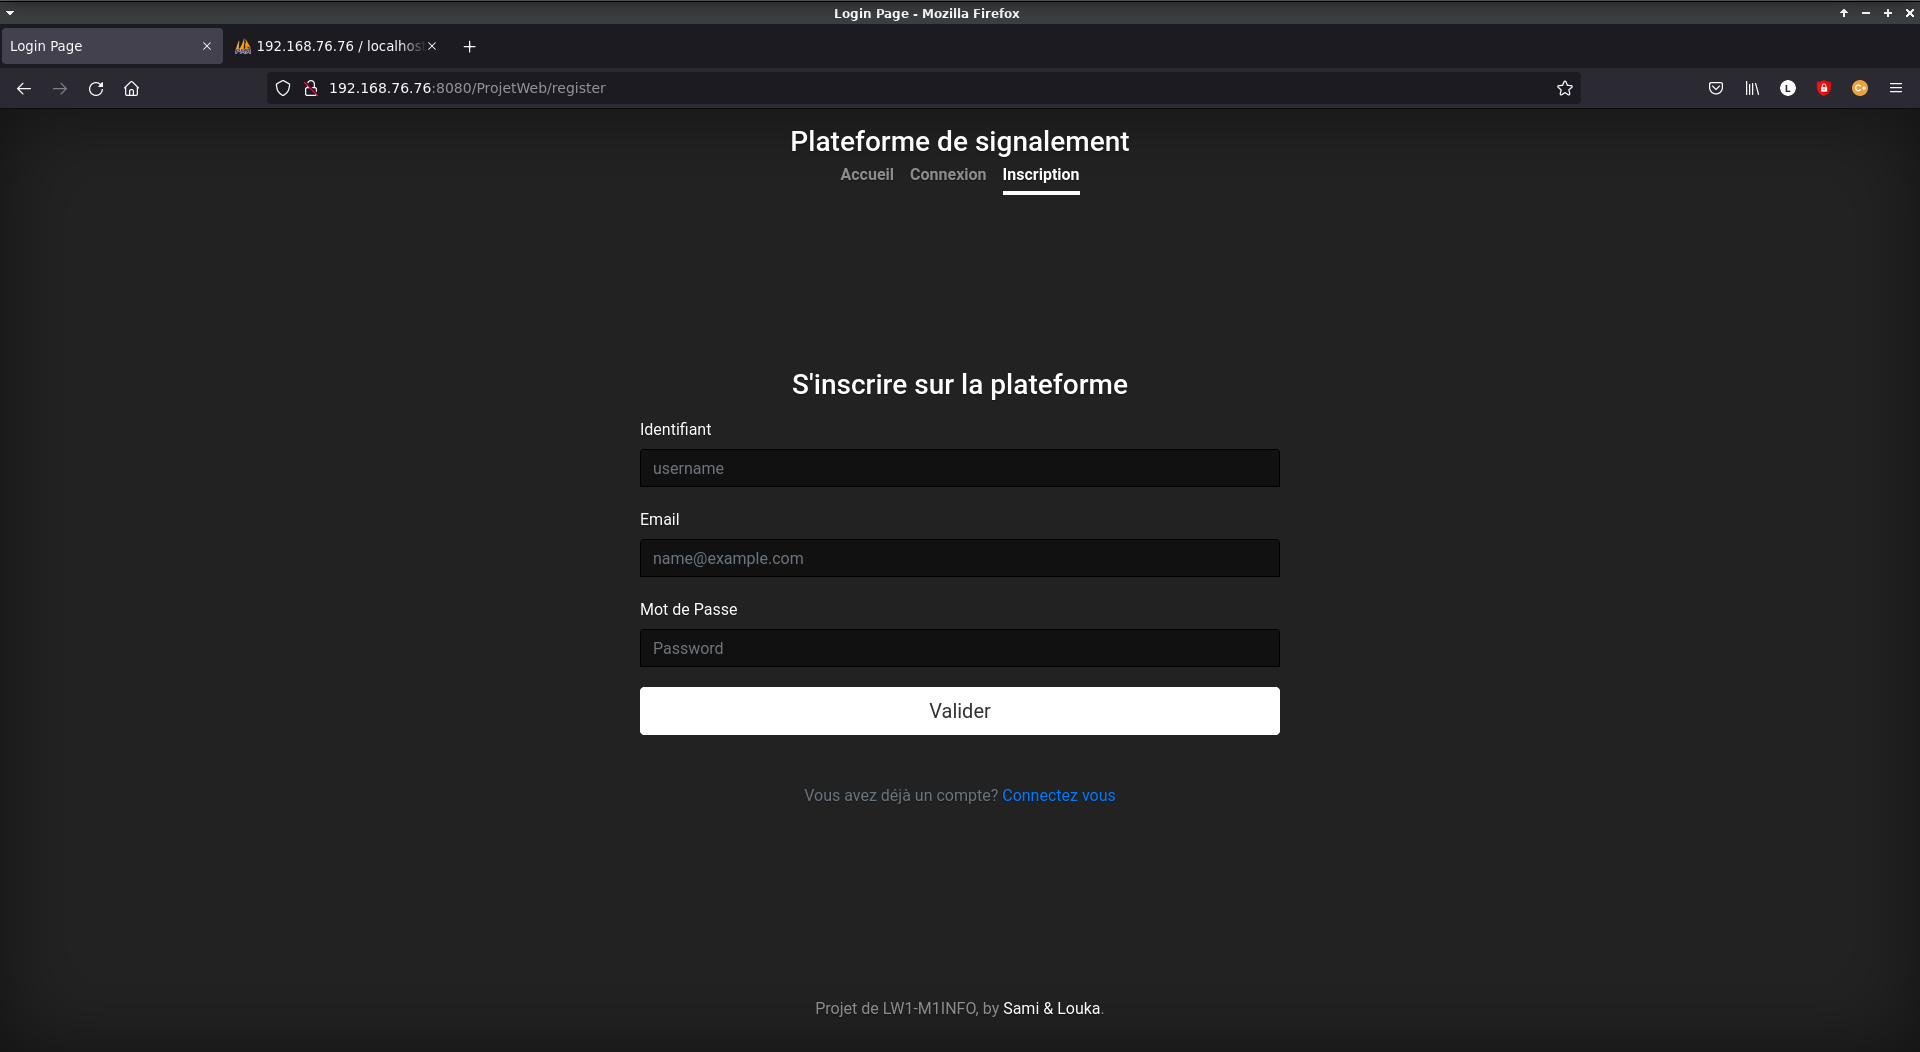
\includegraphics[width=\textwidth]{img/sign-up.png}
    \caption{Page d'inscription}
\end{figure}

Si les informations remplies sont corrects (email correct et mot de passe fort), le compte est
créé. Maintenant pour pouvoir obtenir les droits de responsable de maintenance il faut que
l'administrateur les accordent depuis sa page.

Un mot de passe fort doit faire au moins 8 caractères et contenir au minimum :
\begin{itemize}
    \item Une majuscule,
    \item Une minuscule,
    \item Un chiffre,
    \item Un caractère spécial (!@\#\$\&*).
\end{itemize}
\newpage

Une fois les droits accordés un responsable de maintenance arrive sur la page suivante lorsqu'il
se connecte :
\begin{figure}[!h]
    \centering
    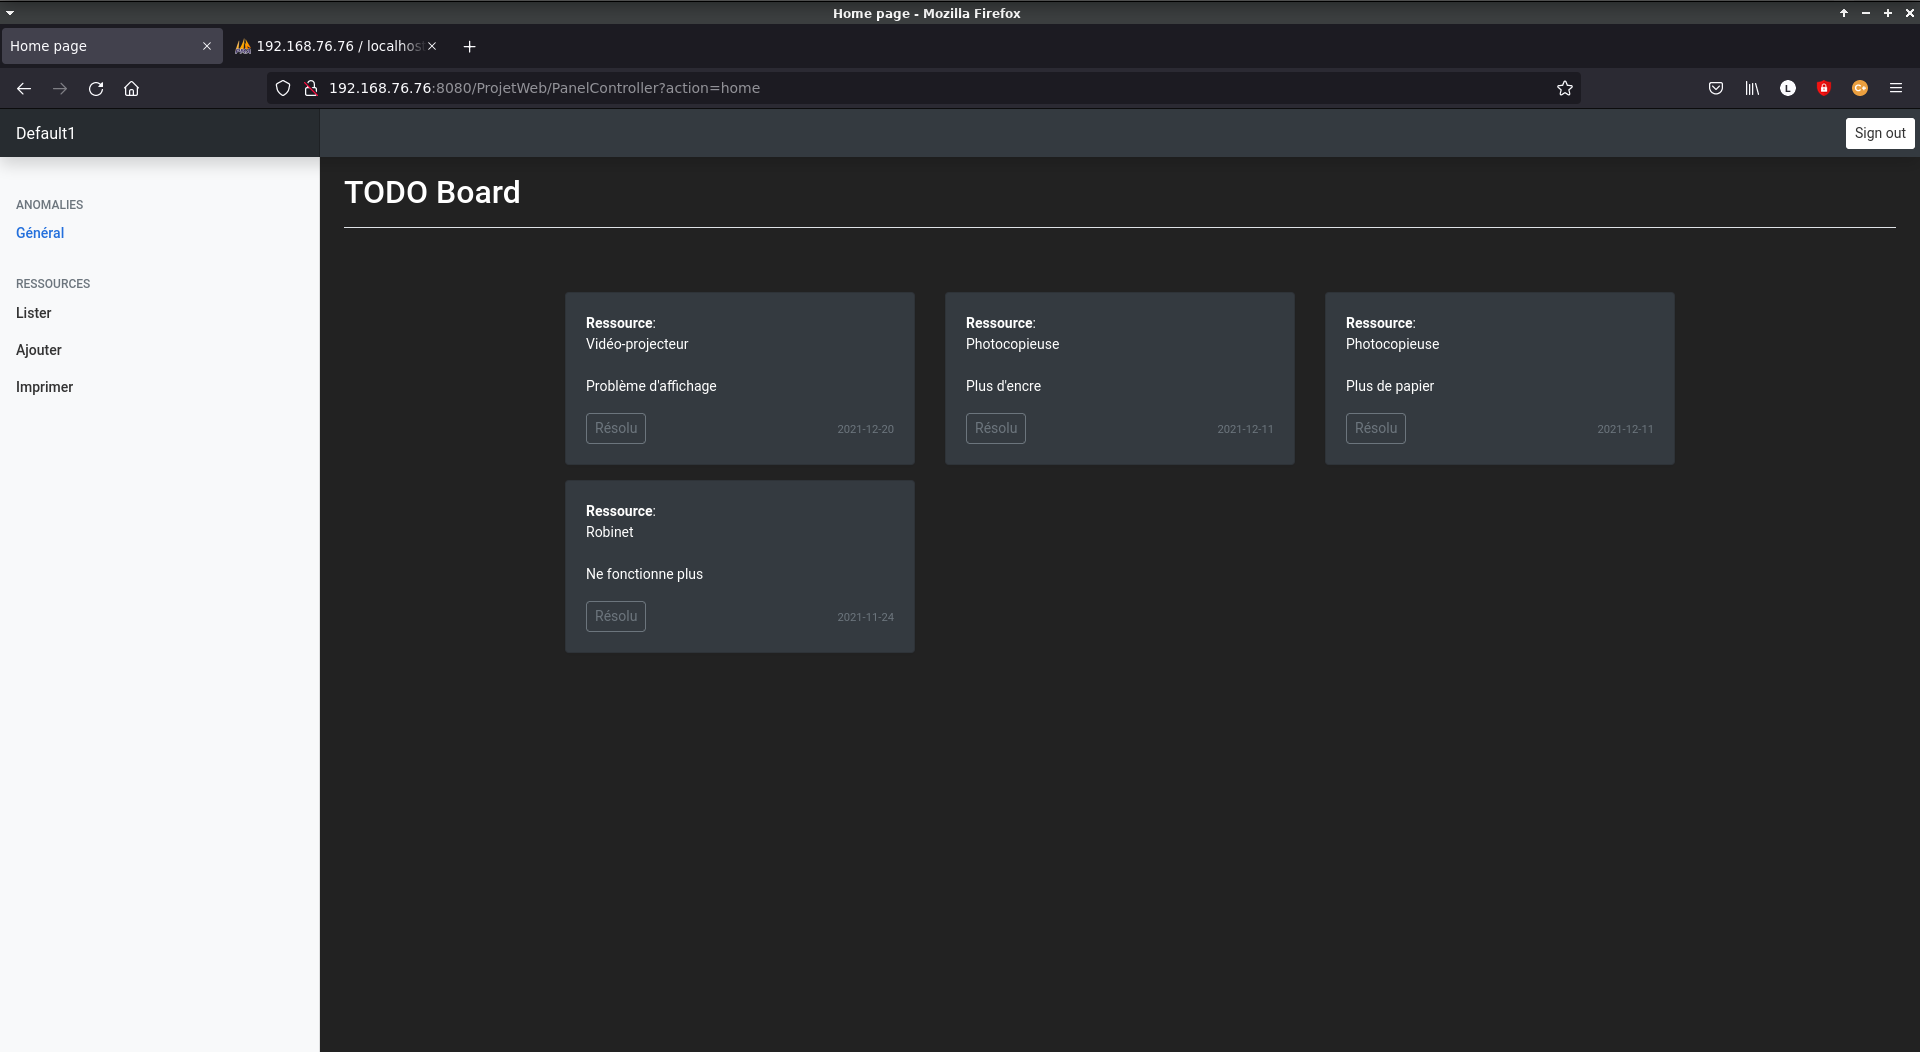
\includegraphics[width=\textwidth]{img/maintainer.png}
    \caption{Panneau de responsable de maintenance}
\end{figure}

Dans le panneau latéral, les actions suivantes sont disponibles :
\begin{description}
    \item[\textbf{Général}] : page principale, affiche la liste des anomalies en attente, non
        résolues.
    \item[\textbf{Lister}] : affiche la liste des ressources dont l'utilisateur est responsable.
    \item[\textbf{Ajouter}] : permet d'ajouter une nouvelle ressource.
    \item[\textbf{Supprimer}] : permet de supprimer une ressource.
\end{description}
Pour chacune des anomalies, lorsque l'une d'elles est résolue, il suffit de cliquer sur
\textbf{Résolu} et son statut change. Sur la page d'accueil on peut voir les dernières anomalies
résolues.
\newpage

Enfin, lorsqu'un utilisateur flash un QR code, par exemple pour la ressource n°1, il arrive sur
la page suivante :
\begin{figure}[!h]
    \centering
    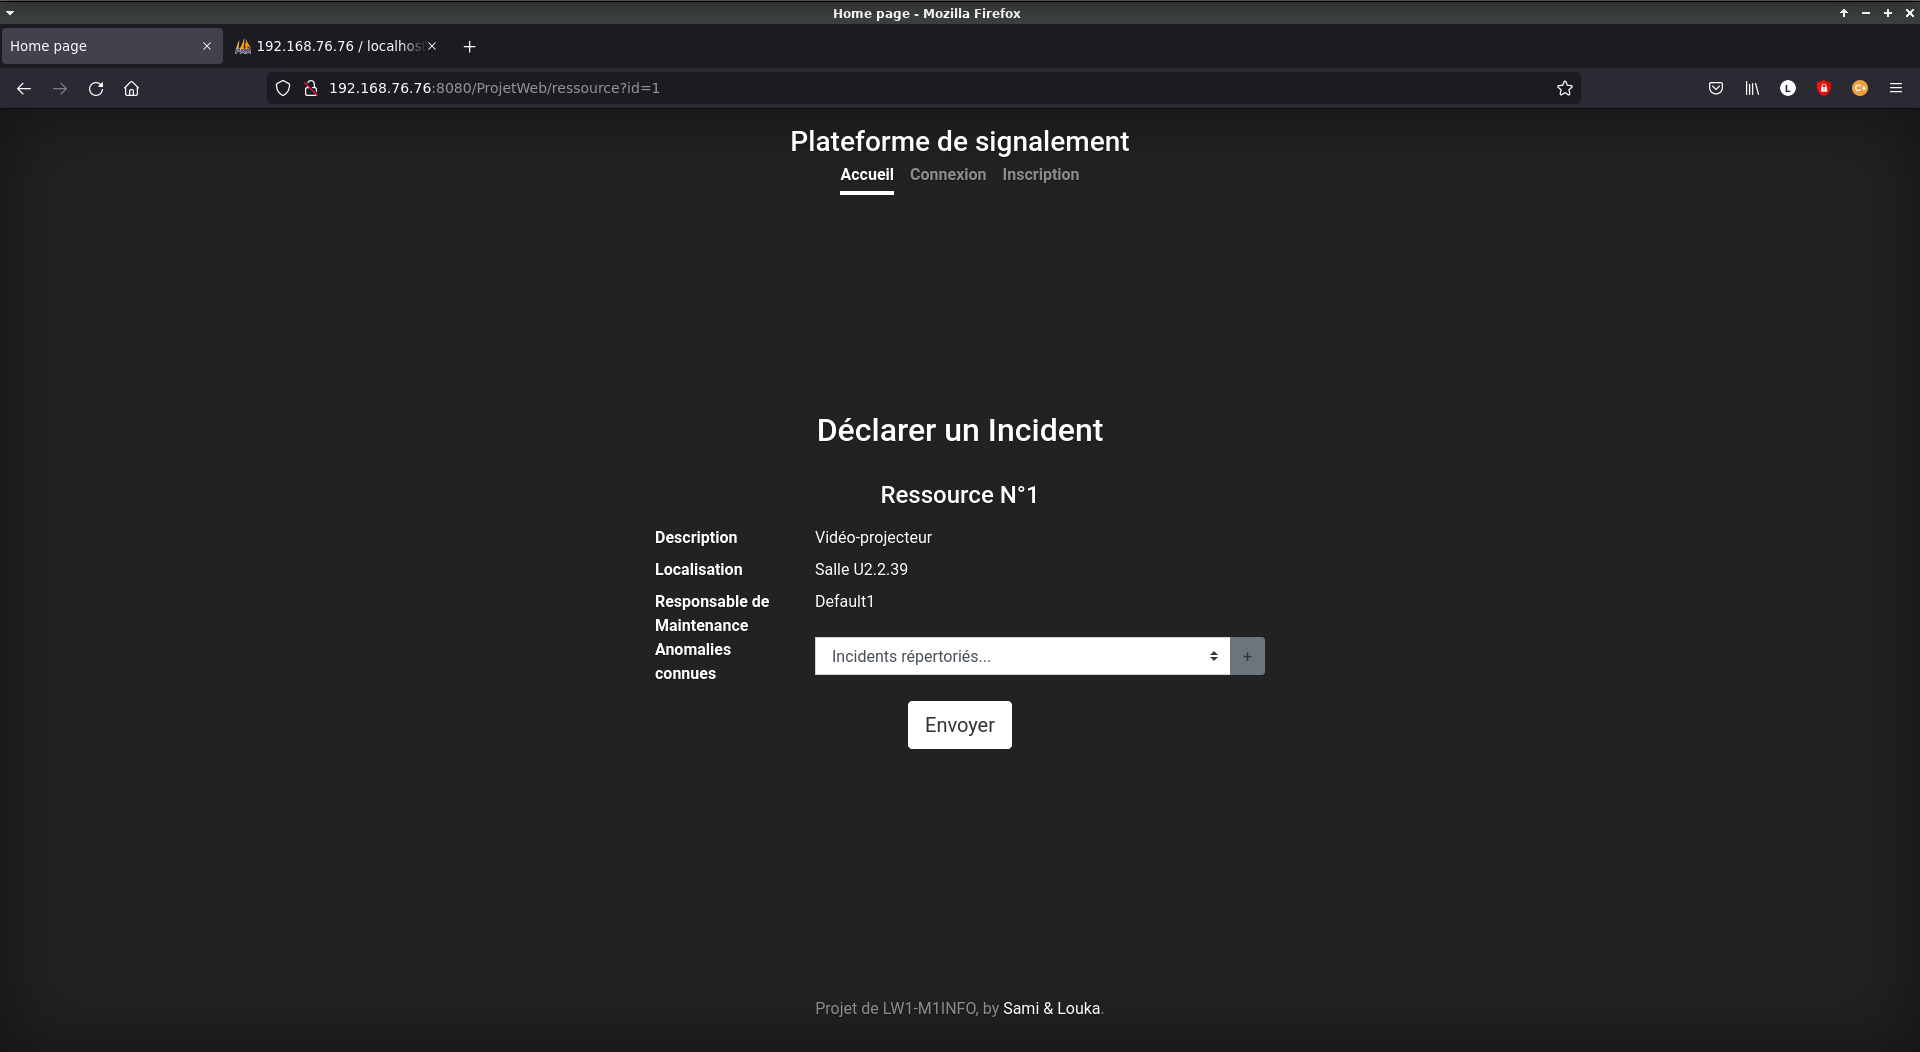
\includegraphics[width=\textwidth]{img/ressource.png}
    \caption{Déclaration d'une anomalie pour le vidéo-projecteur de la salle U2.2.39}
\end{figure}
Il peut donc sélectionner une anomalie déjà signalée dans la liste déroulante
<<Incidents répertoriés>> ou bien cliquer sur le bouton \textbf{+} pour en déclarer une nouvelle.
Ensuite pour la soumettre, il clique sur \textbf{Envoyer}.

